%document
\documentclass[10pt]{beamer}
%theme
\usetheme{metropolis}
% packages
\usepackage{color}
\usepackage{listings}
\usepackage[main=ngerman, USenglish]{babel}
\usepackage[utf8]{inputenc}
\usepackage{multicol}
\usepackage{csquotes}


% color definitions
\definecolor{mygreen}{rgb}{0,0.6,0}
\definecolor{mygray}{rgb}{0.5,0.5,0.5}
\definecolor{mymauve}{rgb}{0.58,0,0.82}
\definecolor{paleorange}{HTML}{CC7832}

\lstset{
    backgroundcolor=\color{white},
    % choose the background color;
    % you must add \usepackage{color} or \usepackage{xcolor}
    basicstyle=\footnotesize\ttfamily,
    % the size of the fonts that are used for the code
    breakatwhitespace=false,
    % sets if automatic breaks should only happen at whitespace
    breaklines=true,                 % sets automatic line breaking
    captionpos=b,                    % sets the caption-position to bottom
    commentstyle=\color{mygreen},    % comment style
    % deletekeywords={...},
    % if you want to delete keywords from the given language
    extendedchars=true,
    % lets you use non-ASCII characters;
    % for 8-bits encodings only, does not work with UTF-8
    frame=single,                    % adds a frame around the code
    keepspaces=true,
    % keeps spaces in text,
    % useful for keeping indentation of code
    % (possibly needs columns=flexible)
    keywordstyle=\color{blue},       % keyword style
    % morekeywords={*,...},
    % if you want to add more keywords to the set
    numbers=left,
    % where to put the line-numbers; possible values are (none, left, right)
    numbersep=5pt,
    % how far the line-numbers are from the code
    numberstyle=\tiny\color{mygray},
    % the style that is used for the line-numbers
    rulecolor=\color{black},
    % if not set, the frame-color may be changed on line-breaks
    % within not-black text (e.g. comments (green here))
    stepnumber=1,
    % the step between two line-numbers.
    % If it's 1, each line will be numbered
    stringstyle=\color{mymauve},     % string literal style
    tabsize=4,                       % sets default tabsize to 4 spaces
    % show the filename of files included with \lstinputlisting;
    % also try caption instead of title
    language = Java,
	showspaces = false,
	showtabs = false,
	showstringspaces = false,
	escapechar = ,
        morecomment=[s][\textcolor{paleorange}]{@}{\ },
}

\def\ContinueLineNumber{\lstset{firstnumber=last}}
\def\StartLineAt#1{\lstset{firstnumber=#1}}
\let\numberLineAt\StartLineAt



\newcommand{\codeline}[1]{
        \alert{\texttt{#1}}
}

\setmonofont{Fira Code}

% This Document contains the information about this course.

% Authors of the slides
\author{Marcus Köhler}

% Name of the Course
\institute{Java-Kurs}

% Fancy Logo
\titlegraphic{\hfill
\includegraphics[height=1.25cm]{../templates/fsr_logo_cropped}}

\usepackage{csquotes}
\usepackage{textcomp}

\begin{document}

\date{\today}

\title{Java}
\subtitle{Recap 2 \tiny{- Electric Boogaloo}}

\begin{frame}
    \titlepage
\end{frame}

\begin{frame}{Übersicht}
    \setbeamertemplate{section in toc}[sections numbered]
    \tableofcontents
\end{frame}

\section{Abstrakte Klassen}
\begin{frame}[fragile]{Abstrakte Klassen}
    \textit{Abstrakte Klassen} sind Klassen, in denen nicht alle Methoden auch eine Definition haben. Das ist praktisch, wenn man in einer Klasse sowohl
    gemeinsames Verhalten als auch sogenannte \textit{Verhaltensvorschriften} (d.h. Vorgabe von Methodensignaturen) haben will. \\
    Abstrakte Klassen \& Methoden sind durch das Keyword \texttt{abstract} gekennzeichnet.
    \onslide<2->
    \begin{lstlisting}[basicstyle=\ttfamily\scriptsize,gobble=8]
        public abstract class UniEmployee {
            private String name;
            private long pNumber;

            public UniEmployee(String name, long pNumber) {
                this.name = name;
                this.pNumber = pNumber;
            }

            public String getName() {return this.name;}
            //abstract because different employees have different salary calculations
            public abstract int calculateSalary();
        }
    \end{lstlisting}
\end{frame}

\begin{frame}[fragile]{Abstrakte Klassen}
    Wichtige Eigenschaften von abstrakten Klassen:
    \begin{itemize}[<+->]
        \item Sie können \textit{nicht} instanziert werden:
            \begin{lstlisting}[basicstyle=\ttfamily\scriptsize,gobble=16]
                UniEmployee employee = new UniEmployee("T. Est", 42);
                //this is not allowed!
            \end{lstlisting}
        \item Erbende Klassen müssen entweder \textit{alle} abstrakten Methoden implementieren ODER auch abstrakt sein:
           \begin{lstlisting}[basicstyle=\ttfamily\scriptsize,gobble=16]
                public abstract class ServiceEmployee extends UniEmployee{ ... }

                public class ResearchEmployee extends UniEmployee {
                    @Override
                    public int calculateSalary { ... }
                }
            \end{lstlisting}
        \item Wenn eine Klasse eine abstrakte Methode enthält, muss sie als abstrakt markiert werden:
            \begin{lstlisting}[basicstyle=\ttfamily\scriptsize,gobble=16]
                public class Truck {
                    public abstract void drive();
                } //this is not permitted, the class must be abstract
            \end{lstlisting}
    \end{itemize}
\end{frame}

\section{Exceptions}
\begin{frame}{Exceptions}
    \textit{Exceptions} sind spezielle Java-Klassen, welche Ausnahmezustände im Verlauf eines Programms darstellen
    und \textit{geworfen} werden, wenn die zugehörigen Zustände eintreten. \\
    Normalerweise beendet eine Exception ein Programm, wenn sie nicht abgefangen und behandelt wird.
    Zustände, in denen Exceptions auftreten, sind u.a.:
    \begin{itemize}[<+->]
        \item Arithmetische Fehler(z.B. Division durch 0)
        \item Ungenügende Ressourcen(z.B. Nicht genug RAM)
        \item Fehlerhafter Programmcode(z.B. Null-Pointer Dereferenzierung)
        \item \dots
    \end{itemize}
\end{frame}

\begin{frame}[fragile]{Exceptions}
    \onslide<+->
    Eine Exception generiert einen sogenannten \textit{Stacktrace} wenn sie geworfen wird. Ein Stacktrace beinhaltet die \enquote{Position} im Programm, in dem die Exception aufgetreten ist.\\
    \onslide<+->
    Ein Stacktrace sieht folgendermaßen aus:
    \begin{lstlisting}[basicstyle=\ttfamily\scriptsize,gobble=8]
        Exception in thread "main" java.lang.NullPointerException
            at com.example.myproject.Book.getTitle(Book.java:16)
            at com.example.myproject.Author.getBookTitles(Author.java:25)
            at com.example.myproject.Bootstrap.main(Bootstrap.java:14)
    \end{lstlisting}
    \onslide<+->
    Im vorangegangenen Beispiel ist die Exception im \texttt{main}-Thread innerhalb der Methode \texttt{Book.getTitle} aufgetreten.\\
    \onslide<+->
    In den Zeilen darunter sind die Methoden aufgelistet, die die jeweils darüberliegende Methode aufgerufen haben.\\
    \onslide<+->
    Die Dateinamen und Zahlen in den Klammern in jeder Zeile geben an, wo genau der Aufruf stattgefunden hat(im Format \textit{<quelldatei:zeile>}).
\end{frame}

\begin{frame}[fragile]{Exceptions}
    \onslide<+->
    Um Exceptions zu behandeln, gibt es in Java den \texttt{try-catch}-Mechanismus. Dieser führt den Code im \texttt{try}-Block aus und fängt jede Exception ab, welche dann im \texttt{catch}-Block behandelt wird. Man kann den \texttt{catch}-Block auch anweisen, nur bestimmmte Arten von Exceptions zu behandeln.
    \onslide<+->
    \begin{lstlisting}[basicstyle=\ttfamily\scriptsize,gobble=8]
        ...
        try {
            int result = numerator/denominator;
        } catch(ArithmeticException e) {
            System.out.println("Illegal division occurred!");
        }
    \end{lstlisting}
    \onslide<+->
    Wenn man selber Exceptions \enquote{werfen} will, kann das mithilfe des \texttt{throw}-Keywords machen.
    \begin{lstlisting}[basicstyle=\ttfamily\scriptsize,gobble=8]
        public void setValue(int val) {
            if(value <= 0) throw new IllegalArgumentException();
            ...
        }
    \end{lstlisting}
\end{frame}

\section{Generics}
\begin{frame}[fragile]{Generics}
    \onslide<+->
    \textit{Generics} sind Javas Implementierung von generischer Programmierung.\\
    \onslide<+->
    Generische Programmierung ist ein Programmierkonzept, welches ermöglicht, verschiedene Ausprägungen einer Klasse bzw. eines Objektes mithilfe einer sogenannten \textit{Typvariable} zu generieren:
    \onslide<+->
    \begin{lstlisting}[basicstyle=\ttfamily\scriptsize,gobble=8]
        public class Node<T> { //T for type
            private T data;
            private Node<T> leftChild, rightChild;
            public Node(T data, Node<T> leftChild, Node<T> rightChild) {...}
            public Node(T data);
            public T getData() { return this.data; }
            public Node<T> getLeftChild() { return this.leftChild; }
        }
    \end{lstlisting}
    \onslide<+->
    In diesem Beispiel ist \texttt{T} die Typvariable der Klasse \texttt{Node}.
    Die Typvariable wird innerhalb der Klasse verwendet, um \enquote{unbekannte} Typen festzulegen und zu garantieren,
    dass diese dem vorgegebenen Typen \texttt{T} entsprechen.
\end{frame}

\begin{frame}[fragile]{Generics}
    \onslide<+->
    Die Typvariablen werden dann bei der Deklaration und Instanzierung konkret festgelegt:
    \onslide<+->
    \begin{lstlisting}[basicstyle=\ttfamily\scriptsize,gobble=8]
        Node<Integer> leftChild = new Node<>(42); //using the <> Operator
        Node<Integer> rightChild = new Node<Integer>(1337); //specifying T in instantiation as well
        Node<Integer> root = new Node<>(10, leftChild, rightChild);
    \end{lstlisting}
    \onslide<+->
    Wenn der Compiler nicht automatisch aus den Argumenten des Konstruktors ableiten kann, welchen Typ die Typvariable annimmt,
    \textbf{muss} T auch im Aufruf des Konstruktors angegeben werden.\\
    \bigskip
    \onslide<+->
    \begin{center}
        \begin{tabular}{l}
            \Large
            >DEMO<\\
        \end{tabular}
    \end{center}
\end{frame}

\section{Collections}
\begin{frame}{Collections}
    \onslide<+->
    Java bietet im Package \texttt{java.util} mit der \textit{Collections-API} Datenstrukturen und Mechanismen an,
    die die Arbeit mit Datensätzen von variabler Größe wesentlich erleichtert.\\
    \onslide<+->
    Arrays sind für solche Datensätze ungeeignet, da man ihre Größe nach der Erstellung nicht mehr ändern kann.\\
    \onslide<+->
    Außerdem legen die verschiedenen Datenstrukturen teilweise auch Beschränkungen auf die in ihnen enthaltenen Daten,
    damit man aufwändige Prüfungen nicht selbst erledigen muss.\\
\end{frame}

\begin{frame}[fragile]{Collections}
    \onslide<+->
    Die Collections-API verwendet Generics, um festzulegen, welchen Typ die enthaltenen Daten haben:
    \begin{lstlisting}[basicstyle=\ttfamily\scriptsize,gobble=8]
        List<String> stringList = new ArrayList<>();
        stringList.add("foo");
        stringList.add("bar");
    \end{lstlisting}
    \onslide<+->
    Außerdem \enquote{erzwingt} die Verwendung von Generics, dass eine Collection nur Elemente des gleichen oder eines erbenden Typs enthält:
    \begin{lstlisting}[basicstyle=\ttfamily\scriptsize,gobble=8]
        Set<Number> numberSet = new HashSet<Number>();
        numberList.add(1.07f);
        numberList.add(0815);
        numberList.add("8998"); //not permitted, as String does not inherit from Number
    \end{lstlisting}
\end{frame}

\begin{frame}[fragile]{Collections}
    \onslide<+->
    Um über die Elemente einer Collection zu iterieren, gibt es in der Collections-API den \texttt{Iterator}.\\
    \onslide<+->
    Ein Iterator für eine Collection kann über die \texttt{iterator()}-Methode der Collection erstellt werden. Das Iterator-Interface definiert u.a. die folgenden Methoden:
    \begin{itemize}[<+->]
        \item hasNext() - [\textcolor{blue}{\texttt{boolean}}] Sind noch Elemente in der Collection vorhanden?
        \item next() - [\texttt{T}] Gibt das nächste Element zurück.
        \item delete() - [\texttt{void}] Entfernt das zuletzt zurückgegebene Element.
    \end{itemize}
    \onslide<+->
    Für einen detaillierten Workflow mit Iterators siehe 07-collections.
\end{frame}

\section{Andere Programmierkonzepte}
\subsection{Casting}

\begin{frame}[fragile]{Casting}
    \onslide<+->
    \textit{Casting} bezeichnet in vielen Programmiersprachen die Umwandlung eines Datentypen in einen anderen, kompatiblen, Datentypen.\\
    In Java kann man zusätzlich ein Objekt in ein anderes Objekt umwandeln, sofern bestimmte Bedingungen erfüllt sind.\footnotemark\\
    \onslide<+->
    Ein Cast hat die folgende Form:
    \begin{lstlisting}[basicstyle=\ttfamily\scriptsize,gobble=8]
        int castedInt = 17;
        float intCast = (float)castedInt;
        System.out.println(intCast); //prints 17.0
    \end{lstlisting}
    \onslide<+->
    Eine wichtige Regel beim Casting ist, dass keine Informationen verloren gehen dürfen.\\
    Deshalb sind Casts wie \texttt{int} \textrightarrow \texttt{float} erlaubt, \texttt{float} \textrightarrow \texttt{int} aber nicht.
    \footnotetext{Für Details siehe 08-progconcepts}
\end{frame}

\subsection{Rekursion}

\begin{frame}{Rekursion}
    \begin{columns}[c]
        \begin{column}{.5\textwidth}
            \onslide<1->{\textit{Rekursion} bezeichnet eine Funktion bzw. eine Lösungsstrategie,
            die sich selbst wieder aufruft, meistens mit einem Subset der ursprünglichen Daten.\\}
            \medskip
            \onslide<2->{Dies passiert so oft, bis entweder ein sogenannter \textit{Basecase} auftritt,
            für den eine Lösung bekannt ist, oder aber keine Lösung gefunden werden kann
            (oder eine \texttt{StackOverflowException} auftritt).}
        \end{column}
        \begin{column}{.5\textwidth}
            \onslide<1->{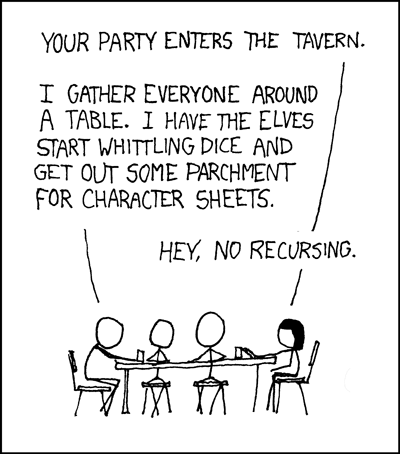
\includegraphics[width=\textwidth]{/home/marcus/git/progcourse/java/images/tabletop_roleplaying.png}
            \tiny{\url{https://xkcd.com/244}}}
        \end{column}
    \end{columns}
\end{frame}

\begin{frame}[fragile]{Rekursion:Beispiel}
    Ein klassisches Beispiel für Rekursion ist eine Funktion, die die n-te Zahl der Fibonacci-Folge berechnet:
    \begin{lstlisting}[gobble=8]
        public int fibonacci(int n) {
            if(n < 0) throw new IllegalArgumentException();
            if(n == 0 || n == 1) return 1; //define basecase
            return fibonacci(n-1) + fibonacci(n-2); //recursive call
        }
    \end{lstlisting}
\end{frame}

\section{JavaDoc}

\begin{frame}{JavaDoc}
    \onslide<+->
    \textit{JavaDoc} ist gleichzeitig die \enquote{Sprache} des Java-Dokusystems und das Tool, mit der die eigentliche Dokumentation generiert wird.
    Javadoc verwendet sogenannte \textit{Tags}, um die Dokumentation zu formatieren.\\
    \onslide<+->
    Dazu wird in einem speziellen mehrzeiligen Kommentar(speziell, weil er mit \texttt{/**} beginnt) mithilfe der Tags Informationen zu Parametern,
    Rückgabewerten etc. aufgeschrieben und anschließend vom Javadoc-Tool formatiert.\\
    \onslide<+->
    Einige übliche Tags und ihre Bedeutung:
    \begin{tabular}{l | l}
            \texttt{@author} & Gibt den Autor an \\
            \texttt{@param} \textit{<name>} & Beschreibung v. Param. \textit{<name>} (nur Methoden)\\
            \texttt{@return} & Beschreibung des Rückgabewertes (nur Methoden) \\
            \texttt{@throws} \textit{<exception>} & Wann \textit{<exception>} auftritt (nur Methoden)\\
            \texttt{\{@code} \textit{<text>}\texttt{\}} & Formatiert \textit{<text>} als Code(d.h. monospaced) \\
        \end{tabular}
\end{frame}

\begin{frame}[fragile]{JavaDoc}
    Eine Javadoc Beschreibung sieht z.B. so aus:
    \begin{lstlisting}[basicstyle=\ttfamily\scriptsize,gobble=8]
        /**
         * Generate a String which is formatted for logging output.
         *
         * @param name The name of the process.
         * @param message The actual message to be printed.
         * @param isError Whether the output should be marked as error.
         *
         * @return A String formatted as "[<time>] <name> <level> <message>"
         */
        public String getLogFormat(String name, String message, boolean isError) {
            String msgLevel = isError ? "CRITICAL" : "INFO";
            String ret = String.format("[%d] %s: %s: %s",
                    System.nanoTime(),  name, msgLevel, message);
            return ret;
        }
    \end{lstlisting}
    \let\thefootnote\relax\footnote{Das Statement \texttt{<expr> ? <true> : <false>} ist eine Kurzform eines if-Statements}
\end{frame}
\end{document}
